% =====================================================================
% VENUE NOTE (read before submitting):
% No AISTATS style file was available in the local template library, and
% fabricating one would silently break formatting compliance. This file is
% therefore written venue-neutrally against `article`. To submit:
%   1. Download the official aistats20XX.sty / .bst from the AISTATS site.
%   2. Replace the \documentclass line and the two \usepackage lines below
%      with the AISTATS preamble; the body needs no changes.
%   3. AISTATS is 8 pages excluding references and appendix.
% =====================================================================
\documentclass[11pt]{article}
\usepackage[margin=1in]{geometry}
\usepackage{amsmath,amssymb,booktabs,graphicx,hyperref,natbib}
\usepackage[T1]{fontenc}

\title{Re-fitting is not Conditioning:\\
A Measured Failure of Return-Conditioned Policies\\
in Multi-Fidelity Bayesian Optimization}
\author{Anonymous Author(s)}
\date{}

\begin{document}
\maketitle

\begin{abstract}
We show that a Decision Transformer trained to act as a multi-fidelity Bayesian
optimization policy does not, in practice, condition on its inputs: across the
realised support of every input channel---the state, the return-to-go, the
budget-to-go, and its own interaction history---the proposed query never
changes. Stretching return-to-go over nine orders of magnitude, far outside
anything the system can present, moves it on $1$ of $12$ probes. Establishing this is difficult because such a policy still
\emph{appears} adaptive---its queries move between iterations---so behavioural
evidence is misleading. We separate the two mechanisms by holding the network's
weights fixed and varying only its inputs, which isolates conditioning from
re-fitting. Across eleven pre-registered interventions spanning the conditioning
architecture, the candidate features, the context length, the return schema, the
reward, the rollout dynamics, and the scoring head, the proposed argmax changes
on $0$ of $12$ probes in every case, and we localize the cause to a
$\sim$10$\times$ attenuation of state variation, split evenly between the
transformer encoder ($0.346\times$) and the scoring head ($0.294\times$).
The most striking number is the sharpest: a full optimization run's worth of
state change---mean pairwise $L_2$ of $1.4968$---rotates the policy's scoring
coefficients by $2.04^\circ$ and changes the decision on zero of twelve
candidate pools.
\end{abstract}

\begin{figure}[t]\centering
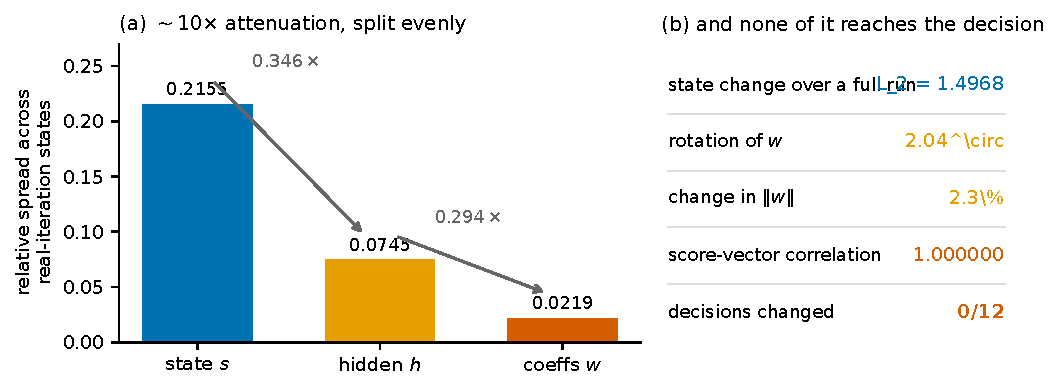
\includegraphics[width=\linewidth]{figs/fig1_mechanism.pdf}
\caption{\textbf{The conditioning channel is inert, and we can say where the
signal is lost.} (a) Relative spread (mean pairwise distance over mean norm) of
each representation across the twelve states of a real optimization run. The
transformer encoder contracts state variation by $0.346\times$ and the scoring
head by a further $0.294\times$, roughly $10\times$ end to end; neither stage
alone is the culprit. (b) The consequence: a full run's worth of state change
rotates the scoring coefficients by $2.04^\circ$, leaves the score vectors
correlated at $1.000000$, and changes the proposed query on none of twelve
independently resampled candidate pools.}
\label{fig:mechanism}
\end{figure}

\section{Introduction}

Return-conditioned supervised learning (RCSL), popularized by the Decision
Transformer \citep{chen2021dt}, casts control as sequence modelling: a
transformer is trained on trajectories annotated with return-to-go (RTG), and at
test time a desired return is supplied to steer behaviour. The approach is
attractive for Bayesian optimization (BO), where a policy could in principle
learn to trade off exploration, exploitation, and---in the multi-fidelity
setting---the choice of which oracle to query.

We study one such method, which we call MF-DRO: a Kennedy--O'Hagan two-fidelity
Gaussian-process ensemble \citep{Kennedy_2000} supplies simulated rollouts, a
Decision Transformer is trained on them, and at each real iteration the
transformer proposes the next $(x, \ell)$ query given a return target and a
budget target.

Our central finding is negative and, we argue, generalizable: \textbf{the policy
never conditions.} It behaves as a per-iteration acquisition function that is
re-fitted from scratch, not as a policy that reads its inputs.

This is easy to miss. The queries do move between iterations---across the ten
frozen-protocol runs, the per-coordinate standard deviation of the query
sequence, averaged over coordinates, spans $0.121$--$0.228$---so any behavioural
test suggests
adaptation. The movement comes entirely from the weights being re-fitted each
iteration, not from the inputs. Separating these requires freezing the weights
and varying only the inputs---which is what we do throughout.

\paragraph{Contributions.}
\begin{itemize}\itemsep2pt
\item \textbf{A measured mechanism, not a black-box null.} We localize the
failure to a $\sim$10$\times$ attenuation of state variation, distributed
$0.346\times$ at the encoder and $0.294\times$ at the scoring head
(Section~\ref{sec:mechanism}). Neither stage alone is the culprit, which
explains why module-specific fixes cannot work.
\item \textbf{Eleven pre-registered interventions, all null.} We vary the
conditioning mechanism, candidate features, context length, RTG schema, reward,
rollout stochasticity, and score-head architecture. The argmax moves on $0/12$
probes in every arm (Section~\ref{sec:interventions}).
\item \textbf{A frozen evaluation that we report as it fell.} Under a protocol
fixed in advance, MF-DRO fails the pre-registered success test with both
rewards, by $0.4481$ and $0.5442$ against a bar of $0.3825$
(Section~\ref{sec:frozen}).
\item \textbf{An instrumentation postmortem.} Three of our own probes were
defective and four auto-generated verdicts were wrong. We report each, because
the failure modes are generic to mechanistic evaluation
(Section~\ref{sec:postmortem}).
\end{itemize}

\section{Setup and Frozen Protocol}
\label{sec:setup}

Section~\ref{sec:setup} fixes the method and the protocol;
Section~\ref{sec:related} places the result against RCSL theory.

\paragraph{Method.} An ensemble of $M{=}10$ Kennedy--O'Hagan GPs models a
high-fidelity (HF) objective $f_H$ and a cheap low-fidelity (LF) proxy $f_L$
with $c_H{=}8$, $c_L{=}1$. Each iteration, $200$ rollouts of length $8$ are
simulated under a Takeno-style multi-fidelity max-value entropy search teacher
\citep{takeno2020mfmes}; the transition $y_\tau$ is a \emph{draw} from the GP
posterior. A Decision Transformer with the four-token layout
$[\textsc{rtg}, \textsc{btg}, s, a]$ per step is trained on these rollouts, then
proposes the next real query by scoring $K{=}200$ uniformly drawn candidates.

\paragraph{Evaluation, frozen before any result was seen.} Hartmann 6D;
baselines MF-MI-Greedy and MF-GP-UCB; $10$ seeds identical across methods;
identical initial design ($36$ HF, $60$ LF); matched real cost ($200$
post-initialization); metric is final simple regret. Success requires
MF-DRO's mean${+}$SE to fall strictly below the best baseline's mean${-}$SE.
The protocol permits the outcome ``no within-frame fix closes the gap''. We
never altered it, and in particular never extended $n$ beyond the ten seeds
fixed in advance.

\paragraph{A prerequisite bug.} An earlier version read all heads from the
\emph{action} token; because the causal mask \texttt{triu(diagonal=1)} permits
self-attention, every head predicted from its own target. Zeroing the action
embedding cost the fidelity head $15.6\%$ of its loss before the fix and $0.7\%$
after. Fixing it eliminated an incumbent-freeze pathology ($0/10$ frozen runs
versus $9/12$ before). \textbf{All results here are post-fix}; pre-fix numbers
are not comparable and are excluded.

\section{The Conditioning Channel Is Inert}
\label{sec:mechanism}

We hold the trained weights fixed and vary only the inputs. Unless stated, a
probe reports the fraction of $12$ independently resampled candidate pools on
which the proposed argmax changes.

Budget-to-go is inert across its realised support $[22,52]$ ($0/12$, correlation
$1.000000$) and remains so at $\{5,100,500\}$. Return-to-go is inert in-band
($0/12$) and moves the argmax on $1/12$ only when swept from $10^{-3}$ to
$10^{6}$. We state this precisely rather than claiming absolute invariance: no
in-distribution value of either channel changes the decision, and a $10^{9}$-fold
stretch of RTG changes it on $8.3\%$ of probes, well below the $30\%$ bar used
throughout.

\paragraph{The state does not move the decision.} Comparing hidden states from
genuinely distinct inputs, the argmax changes on $0/12$ pools and the score
vectors correlate at $1.000000$. This holds both across ensemble members at a
fixed iteration and---more importantly---across the twelve states of a real
optimization run, whose mean pairwise $L_2$ distance is $1.4968$.

One of the two state-dependent quantities the architecture exposes at the
decision is moreover irrelevant \emph{by construction}: $b(h)$ adds the same
constant to every candidate and therefore cannot change an argmax, which we
confirm empirically ($0/12$).

\paragraph{Where the signal is lost.} Table~\ref{tab:atten} tracks the relative
spread (mean pairwise distance divided by mean norm) of each representation
across the twelve real-iteration states; Figure~\ref{fig:mechanism} plots it.

\begin{table}[t]\centering
\caption{Attenuation of state variation through the network. The loss is
distributed, not localized: roughly $3\times$ at the encoder and $3\times$ again
at the scoring head.}
\label{tab:atten}
\begin{tabular}{lcc}
\toprule
Stage & Relative spread & Attenuation \\
\midrule
state $s$            & 0.2155 & --- \\
hidden $h$ (encoder) & 0.0745 & $0.346\times$ \\
coefficients $w$ (head) & 0.0219 & $0.294\times$ \\
\bottomrule
\end{tabular}
\end{table}

End-to-end this is a $\sim$10$\times$ contraction. Concretely, a full run's
worth of state change rotates the scoring coefficient vector by $2.04^\circ$
(minimum pairwise cosine $0.99936628$) and changes its norm by $2.3\%$---far too
small to reorder $200$ candidates. The fidelity head is equally inert: with
weights fixed, its output spans only $0.1248$--$0.1286$ across the whole run.

\paragraph{The two stages have different causes.} Comparing the trained network
against a randomly initialised one with identical architecture, identical states
and identical pools separates learning from shape. The encoder's contraction is
\emph{architectural}: a random transformer contracts state variation by
$0.4601\times$ against the trained network's $0.3898\times$, a ratio of only
$1.18$. The head's contraction is \emph{learned}, and dramatically so: a random
head \emph{amplifies} variation ($1.6039\times$) where the trained head contracts
it ($0.3348\times$)---a $4.8\times$ swing attributable entirely to fitting.

Training therefore collapses the scoring head, while the encoder was never
passing much through to begin with. The two stages need different remedies and
should not be treated as one phenomenon.

Neither, however, is close to the threshold that would matter---and we can say
how far. Holding the trained network fixed and scaling state deviations as
$s'(\lambda) = \bar{s} + \lambda(s-\bar{s})$ for $\lambda$ up to $100$, the
argmax never moves on more than one of twelve pools, and the single exception at
$\lambda{=}60$ is non-monotonic. The manipulation is not a no-op: across the
sweep the coefficient vector's relative spread grows $76\times$
($0.001826 \to 0.138267$) and $w$ rotates to cosine $0.97988$, an $11.5^\circ$
separation. \textbf{The learned map is invariant to state direction across two
orders of magnitude of input gain.} We verified the reason directly rather than
inferring it. Decomposing $w(s) = \bar{w} + \delta(s)$ over the ten states,
scoring with $\bar{w}$ \emph{alone} reproduces the full model's argmax on
$12/12$ pools; the top-1/top-2 margin exceeds anything $\delta(s)$ can
contribute by a median factor of $77$; and
$\|\delta\|/\|\bar{w}\| = 0.00129$. \textbf{The state moves the coefficient
vector by $0.13\%$ of its length.} MF-DRO's learned policy is, to within a tenth
of a percent, a \emph{fixed linear acquisition function}---not a policy that
conditions weakly, but a constant rule with a negligible state-dependent
perturbation superimposed. (Large $\lambda$ is far out of distribution; this
characterises the map's gain and is not proposed as an intervention.)
(These figures are measured over ensemble-member states, whose spread is
$0.013993$; Table~\ref{tab:atten} is measured over real-iteration states, about
$15\times$ more varied. The two are consistent in magnitude but are different
state sets.) Section~\ref{sec:interventions} tests an unbottlenecked head
directly.

\subsection{The rule it converges to is uncertainty-averse}
\label{sec:rule}

If the policy is a fixed linear rule, it is fair to ask which one. Its signed
coefficients are dominated by the two posterior means---$\mu_H$ at $+1.0824$ and
$\mu_L$ at $+0.8254$---followed by a term that should not be there:

\begin{center}
$\bar{w}_{\sigma_H} < 0$ on $\mathbf{9}$ of $\mathbf{10}$ independently trained
seeds; mean $\mathbf{-0.2544}$ (sd $0.2578$)
\end{center}

\noindent
\textbf{The weight on high-fidelity posterior uncertainty is negative.} The
learned rule \emph{penalises} exactly the quantity that UCB, EI and MES reward,
converging to a purely exploitative, actively
uncertainty-avoiding acquisition. All ten seeds reward $\mu_H$; nine of ten
penalise $\sigma_H$. The \emph{sign} is robust; the \emph{magnitude} is not,
spanning $-0.6871$ to $+0.1297$ with a mean about one standard deviation from
zero, so we report the distribution rather than any one model's coefficient.

An independent check confirms the sign without relying on any single rule
matching. Sweeping a UCB family $\mu_H + \beta\sigma_H$, agreement with the
learned argmax falls monotonically as the exploration bonus grows:
$66.7\%$ at $\beta{=}1$, $50.0\%$ at $\beta{=}2$, $41.7\%$ at $\beta{=}3$,
$25.0\%$ at $\beta{=}5$.

We deliberately do \emph{not} name the rule. The best single match reaches
$75.0\%$ on twelve pools and two candidate rules tie there, which is far too
weak to support an identity claim. The coefficient table and the monotone sweep
are the robust results.

This supplies the causal link to Section~\ref{sec:frozen}. A rule that penalises
HF uncertainty concentrates queries where the model is already confident,
gathering little new information and improving the incumbent slowly---the
pathology this investigation began from.

The aversion is \textbf{inherited, not learned wrong}. Over $1600$ teacher
decisions, the MF-MES teacher's own choices sit at the $2.9$th percentile of
$\sigma_H$ within their candidate pools (control: the $94.2$nd percentile of
$\mu_H$). Its \emph{score} does mildly reward uncertainty
(Spearman $+0.1585$ with $\sigma_H$), but its \emph{argmax} is dominated by the
posterior mean (Spearman $+0.8517$), and in a GP the high-$\mu$ region is
precisely where data already sits. So MF-MES's realised behaviour on this
benchmark is exploitative even though its scoring rule is not, and a student
trained to imitate \emph{choices} can only learn the exploitative part.

This relocates the fault: a better student cannot repair an exploitative teacher.
And the teacher's exploitativeness is \textbf{intrinsic, not a tuning artefact}.
Sweeping the cost ratio over $\{2,4,8,16\}$ and the $y^\ast$ sample count over
$\{5,10,50\}$, the chosen-$\sigma_H$ percentile never exceeds $5.5\%$ in any of
the twelve cells (control $93.6$--$94.7\%$ throughout). Ten times more Monte
Carlo changes nothing, and an $8\times$ swing in the cost ratio moves the
percentile only from ${\sim}1\%$ to ${\sim}5\%$.

The conclusion is therefore structural rather than incidental: \emph{a student
trained to imitate the choices of an argmax-of-MES teacher cannot learn to
explore at any operating point we tested}. Remedying it requires learning from
the teacher's \emph{scores} over the full candidate set rather than its argmax,
or an explicitly exploration-augmented demonstrator---not a better student and
not a different cost ratio.

\section{Eleven Interventions}
\label{sec:interventions}

\begin{figure}[t]\centering
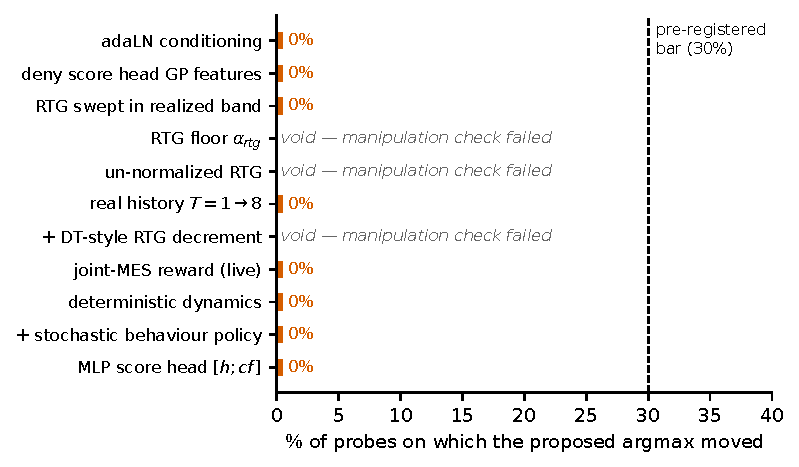
\includegraphics[width=.78\linewidth]{figs/fig2_interventions.pdf}
\caption{Eleven pre-registered interventions on the conditioning pathway. Bars
show the fraction of probes on which the proposed argmax changed; every arm is
at zero against a pre-registered success bar of $30\%$. Three arms are marked
void: they failed their own manipulation checks and are not interpreted.}
\label{fig:interventions}
\end{figure}

\begin{table}[t]\centering
\caption{Pre-registered interventions on the conditioning pathway. ``Void''
means the intervention failed its own manipulation check and was not
interpreted.}
\label{tab:interventions}
\begin{tabular}{llc}
\toprule
& What was changed & Argmax moved \\
\midrule
H4  & adaLN conditioning \citep{peebles2023dit,wang2026ddt} & $0/12$ \\
H5  & deny score head its GP features & $0/12$ \\
H8  & sweep RTG within its realized band & $0/12$ \\
H9  & RTG floor $\alpha_{\mathrm{rtg}}$ & void \\
H10 & un-normalized RTG & void \\
H11 & real history, $T{=}1 \rightarrow T{=}8$ & $0/12$ \\
H11c& + DT-style RTG decrement & void \\
H17 & joint-MES reward (live signal) & $0/12$ \\
H19 & deterministic rollout dynamics & $0/12$ \\
H19b& + stochastic behaviour policy & $0/12$ \\
H20 & MLP score head over $[h;\mathit{cf}]$ & $0/12$ \\
\bottomrule
\end{tabular}
\end{table}

Table~\ref{tab:interventions} and Figure~\ref{fig:interventions} summarize all
eleven. Three results deserve emphasis.

\paragraph{The RTG band was capped by algebra.} The target
$\max(\text{batch\_max}, \alpha\cdot\text{running\_max})$ with
$\text{batch\_max}\le\text{running\_max}$ admits a band of at most $1/\alpha$.
At $\alpha{=}0.5$ this is $2\times$, whatever the reward. Two experiments (H9,
H10) were spent against this ceiling before we derived it; both voided on their
own manipulation checks, measuring $1.76\times$ and $2.59\times$.

\paragraph{The reward was dead, and fixing it did not restore conditioning.}
Under an improvement-based reward, an LF step earns \emph{exactly} zero, so
$63.0\%$ of training trajectories carried a return of $0$. Switching to the
joint set-level information gain
$\log b_0 - \log b_T = H[y^\ast|D_0]-H[y^\ast|D_T]$ eliminates this ($0.0\%$
dead, $100\%$ of LF steps credited, CV $0.66$ versus $1.96$) and measurably
improves teacher-quality correlation (paired $+0.0962$, $8/10$ seeds, Wilcoxon
$p{=}0.0195$). The argmax still moves $0/12$.

\paragraph{Removing the head's bottleneck does not help.} Replacing the linear
scoring rule $\langle w(h), \mathit{cf}_k\rangle + b(h)$ with an MLP over
$[h;\mathit{cf}_k]$---verified non-affine, residual $0.0863$ against the linear
head's $0.000000$---still yields $0/12$. The failure is architecture-independent
within this family, exactly as the encoder-side attenuation predicts.

\section{Frozen Evaluation}
\label{sec:frozen}

\begin{figure}[t]\centering
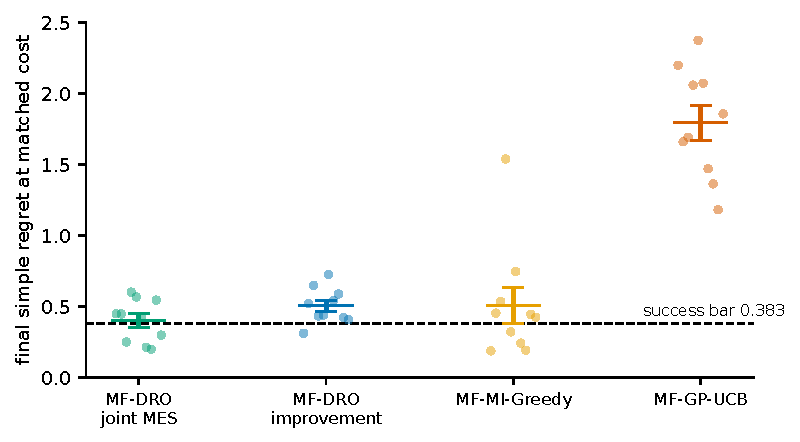
\includegraphics[width=.72\linewidth]{figs/fig3_frozen.pdf}
\caption{Frozen evaluation, ten seeds. Points are individual seeds; bars are
mean $\pm$ SE. Both MF-DRO arms sit above the pre-registered success bar (best
baseline mean${-}$SE). The joint-MES arm has the lowest mean of any method and
the difference is not significant (Wilcoxon $p{=}0.432$ against MF-MI-Greedy).}
\label{fig:frozen}
\end{figure}

\begin{table}[t]\centering
\caption{Final simple regret at matched cost ($\approx 200$), $10$ seeds.
Lower is better. Both MF-DRO arms fail the pre-registered success test
(mean${+}$SE $<0.3825$).}
\label{tab:frozen}
\begin{tabular}{lcc}
\toprule
Method & Final simple regret & sd \\
\midrule
MF-DRO / joint MES     & $\mathbf{0.4007 \pm 0.0475}$ & 0.150 \\
MF-DRO / improvement   & $0.5047 \pm 0.0395$ & 0.125 \\
MF-MI-Greedy           & $0.5091 \pm 0.1266$ & 0.400 \\
MF-GP-UCB              & $1.7934 \pm 0.1223$ & 0.387 \\
\bottomrule
\end{tabular}
\end{table}

Table~\ref{tab:frozen} and Figure~\ref{fig:frozen} report the outcome. The
joint-MES reward gives the lowest mean of any arm, below both baselines,
with $2.7\times$ smaller dispersion than MF-MI-Greedy. \textbf{None of this is
statistically significant.} Paired against MF-MI-Greedy the difference is
$-0.1085$ on $6/10$ seeds (Wilcoxon $p{=}0.432$); against the improvement reward
it is $-0.1040$ on $6/10$ ($p{=}0.375$). Per-seed differences span $-0.399$ to
$+0.169$. The paired standard deviation of $0.2339$ implies roughly $40$ seeds
for $80\%$ power.

We did not run $40$ seeds. The protocol fixes $n{=}10$, and extending it after
seeing a favourable mean is precisely the optional stopping a frozen protocol
exists to prevent. The pre-registered answer is a failure, and we report it.

The only significant win is over MF-GP-UCB ($p{=}0.002$), which under this cost
ratio never queries HF at all ($n_{\mathrm{HF}}{=}0$ on all ten seeds), so its
incumbent cannot move by construction. Beating it is not evidence of much.

\paragraph{Interpretation.} The one intervention that moved regret changed the
\emph{training signal}, not the conditioning pathway---which is what an inert
conditioning channel predicts. MF-DRO improves the way a re-fitted acquisition
function improves.

\section{Why Conditioning Fixes Cannot Rescue This}
\label{sec:related}

\citet{brandfonbrener2022rcsl} give necessary conditions for RCSL to recover an
optimal policy: near-deterministic dynamics, adequate return coverage
$P_\beta(g{=}f(s)|s)\ge\alpha_f$, and a conditioning function equal to the
optimal value function. Their bound scales as
$\epsilon(1/\alpha_f + 3)H^2$, and---most relevant here---they exhibit an MDP in
which the RCSL bias persists \emph{regardless of the conditioning function}.

Our setting violates two conditions by construction. The rollout transition is a
draw from a GP posterior, so $\epsilon$ is large; and the dead-reward
measurement above ($63\%$ of returns identically zero) is small $\alpha_f$ in
their language. This explains why the conditioning-side interventions in
Table~\ref{tab:interventions} were bound to fail.

\textbf{But it is not the whole story, and we tested that.} Making the dynamics
deterministic (H19; verified, repeat-difference $0.000000$) with diversity
intact ($200/200$ distinct trajectories) still yields $0/12$. Near-determinism
is therefore not the binding constraint in MF-DRO; the architecture is. This
also means our refutation of adaLN-style conditioning (H4), following the
diagnosis of scarce attention to return tokens \citep{tanaka2024radt} and the
decoupling remedy of \citet{wang2026ddt}, should be read narrowly: those
mechanisms address a channel that is downstream of where our signal is already
lost.

A constructive direction we did not pursue is dichotomy-of-control
\citep{yang2022doc}, which conditions on a latent that excludes what the policy
cannot influence---in our setting, the fantasy draw.

\section{Instrumentation Postmortem}
\label{sec:postmortem}

We report our own measurement failures because they are generic to this kind of
work, and because two of them would have changed our conclusions.

\begin{itemize}\itemsep2pt
\item \textbf{A probe that compared a state with itself.} Our state-swap test
drew its comparison from indices $7$--$18$ of a batch built as
\texttt{for model: for rollout in range(20)}, so all twelve comparisons shared
one $\tau{=}0$ state. Verified: $12/12$ identical. The conclusion survived
re-measurement with genuinely distinct states, but the original evidence was
worthless.
\item \textbf{A diversity metric that omitted the variable of interest.} A
trajectory signature of (return, fidelity pattern) with no query locations
made rollouts with a dead reward look identical. It produced a structural claim
about coupled failure conditions that we withdrew once locations were included
($200/200$ distinct in every arm).
\item \textbf{A flag that was never wired.} \texttt{use\_linear\_score\_head}
was never forwarded into the model config, so its \texttt{False} branch had been
unreachable since it was written. An \texttt{assert} inside the probe caught it;
without that assert we would have reported a confident null from an arm
identical to the control.
\item \textbf{Four auto-generated verdicts were wrong}, each keyed on a proxy
rather than the decisive quantity: a null-guard that fired without requiring its
manipulation check to pass; a metric that saturated at $100\%$ in both compared
arms; the signature above; and a cosine threshold used in place of argmax
movement. In every case the underlying data were fine and the generated sentence
was not.
\end{itemize}

The transferable rules: derive the reachable range of a formula you control
before experimenting on it; run manipulation checks first, as standalone gates,
with a commitment to stop; assert inside a probe that the manipulation took
effect; and never let an automated verdict key on a proxy.

\section{Limitations}

Our claims are established on \emph{one} benchmark (Hartmann 6D), one method
family, and $n{=}10$ seeds fixed by the frozen protocol. The regret comparison
is underpowered by roughly a factor of four, so we can state that MF-DRO does
not clear the pre-registered bar but not that it is equivalent to MF-MI-Greedy.
The attenuation measurement is taken at the end of training on trained weights;
we did not track it through training. We show that an unbottlenecked scoring
head does not restore conditioning; a random-initialisation control shows the
encoder's share of the contraction is architectural rather than learned; and a
gain sweep shows no threshold within $100\times$. We did not attempt
architectural remedies that change capacity rather than gain (a wider hidden
state, or a scoring rule whose ranking is not dominated by a state-independent
component), so ``the conditioning channel in this trained system is unusable''
remains better supported than ``no architecture in this family could
condition''.
Finally, the pre-fix results are excluded rather than re-run, so we cannot say
how much of the original method's reported behaviour was leakage.

\section{Conclusion}

A Decision Transformer used as a multi-fidelity BO policy can look adaptive
while conditioning on nothing. We measured the failure rather than inferring it:
a $\sim$10$\times$ attenuation of state variation leaves the proposed query
invariant under every input we can vary, including its own history and a
$1.4968$-magnitude change in state. Eleven pre-registered interventions do not
move it, a frozen evaluation fails with both rewards, and the single change that
improved regret did so by improving what the network re-fits toward. For
practitioners, the operational test is simple and we recommend it: freeze the
weights, vary the inputs, and check whether the decision changes at all.

\bibliographystyle{plainnat}
\bibliography{refs}

\end{document}
